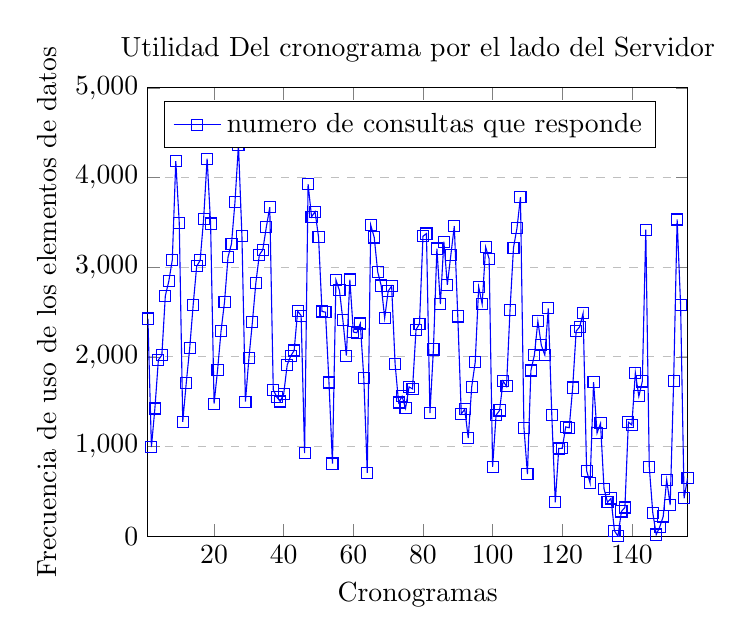
\begin{tikzpicture}
\begin{axis}[
    title={Utilidad Del cronograma por el lado del Servidor},
    xlabel={Cronogramas},
    ylabel={Frecuencia de uso de los elementos de datos},
    xmin=1, xmax=156,
    ymin=0, ymax=5000,
    xtick={},
    ytick={},
    legend pos=north west,
    ymajorgrids=true,
    grid style=dashed,
]

\addplot[
    color=blue,
    mark=square,
    ]
    coordinates {
%UTILIDAD TOTAL
(1,2427)
(2,995)
(3,1424)
(4,1966)
(5,2019)
(6,2681)
(7,2844)
(8,3081)
(9,4184)
(10,3493)
(11,1276)
(12,1706)
(13,2097)
(14,2581)
(15,3010)
(16,3076)
(17,3540)
(18,4211)
(19,3487)
(20,1478)
(21,1851)
(22,2287)
(23,2612)
(24,3112)
(25,3260)
(26,3726)
(27,4363)
(28,3350)
(29,1500)
(30,1983)
(31,2385)
(32,2825)
(33,3137)
(34,3195)
(35,3446)
(36,3669)
(37,1633)
(38,1553)
(39,1502)
(40,1588)
(41,1910)
(42,2008)
(43,2071)
(44,2510)
(45,2460)
(46,926)
(47,3927)
(48,3562)
(49,3620)
(50,3338)
(51,2506)
(52,2499)
(53,1714)
(54,810)
(55,2857)
(56,2743)
(57,2409)
(58,2014)
(59,2862)
(60,2277)
(61,2269)
(62,2372)
(63,1768)
(64,707)
(65,3469)
(66,3332)
(67,2947)
(68,2795)
(69,2433)
(70,2733)
(71,2790)
(72,1918)
(73,1491)
(74,1559)
(75,1427)
(76,1665)
(77,1643)
(78,2303)
(79,2369)
(80,3345)
(81,3375)
(82,1372)
(83,2083)
(84,3208)
(85,2589)
(86,3285)
(87,2804)
(88,3134)
(89,3459)
(90,2451)
(91,1363)
(92,1416)
(93,1093)
(94,1665)
(95,1940)
(96,2780)
(97,2589)
(98,3224)
(99,3094)
(100,774)
(101,1351)
(102,1402)
(103,1730)
(104,1672)
(105,2522)
(106,3218)
(107,3435)
(108,3782)
(109,1211)
(110,693)
(111,1848)
(112,2019)
(113,2397)
(114,2128)
(115,2020)
(116,2541)
(117,1353)
(118,377)
(119,978)
(120,981)
(121,1219)
(122,1209)
(123,1658)
(124,2287)
(125,2334)
(126,2486)
(127,731)
(128,593)
(129,1719)
(130,1150)
(131,1258)
(132,530)
(133,378)
(134,421)
(135,60)
(136,0)
(137,276)
(138,320)
(139,1272)
(140,1240)
(141,1823)
(142,1559)
(143,1726)
(144,3418)
(145,775)
(146,263)
(147,18)
(148,102)
(149,220)
(150,629)
(151,348)
(152,1729)
(153,3532)
(154,2574)
(155,422)
(156,647)
    };
    \legend{numero de consultas que responde}

\end{axis}
\end{tikzpicture}

